\documentclass[
11pt, % The default document font size, options: 10pt, 11pt, 12pt
%codirector, % Uncomment to add a codirector to the title page
]{plan}




% El títulos de la memoria, se usa en la carátula y se puede usar el cualquier lugar del documento con el comando \ttitle
\titulo{Cámara IoT para Detección Facial con conectividad Wi-Fi}

% Nombre del posgrado, se usa en la carátula y se puede usar el cualquier lugar del documento con el comando \degreename
%\posgrado{Carrera de Especialización en Sistemas Embebidos}
%\posgrado{Carrera de Especialización en Internet de las Cosas}
%\posgrado{Carrera de Especialización en Intelegencia Artificial}
\posgrado{Maestría en Sistemas Embebidos}
%\posgrado{Maestría en Internet de las cosas}

% Tu nombre, se puede usar el cualquier lugar del documento con el comando \authorname
\autor{Esp. Ing. Mauricio Barroso Benavides}

% El nombre del director y co-director, se puede usar el cualquier lugar del documento con el comando \supname y \cosupname y \pertesupname y \pertecosupname
\director{Mg. Ing. Gonzalo Sanchez}
\pertenenciaDirector{FF.AA, FIUBA}
% FIXME:NO IMPLEMENTADO EL CODIRECTOR ni su pertenencia
\codirector{John Doe} % para que aparezca en la portada se debe descomentar la opción codirector en el documentclass
\pertenenciaCoDirector{FIUBA}

% Nombre del cliente, quien va a aprobar los resultados del proyecto, se puede usar con el comando \clientename y \empclientename
\cliente{Nombre del cliente}
\empresaCliente{Empresa del cliente}

% Nombre y pertenencia de los jurados, se pueden usar el cualquier lugar del documento con el comando \jurunoname, \jurdosname y \jurtresname y \perteunoname, \pertedosname y \pertetresname.
\juradoUno{Nombre y Apellido (1)}
\pertenenciaJurUno{pertenencia (1)}
\juradoDos{Nombre y Apellido (2)}
\pertenenciaJurDos{pertenencia (2)}
\juradoTres{Nombre y Apellido (3)}
\pertenenciaJurTres{pertenencia (3)}
\fechaINICIO{23 de junio de 2021}		%Fecha de inicio de la cursada de GdP \fechaInicioName
\fechaFINALPlan{11 de agosto de 2021} 	%Fecha de final de cursada de GdP
\fechaFINALTrabajo{15 de diciembre de 2022}	%Fecha de defensa pública del trabajo final


\begin{document}

\maketitle
\thispagestyle{empty}
\pagebreak


\thispagestyle{empty}
{\setlength{\parskip}{0pt}
\tableofcontents{}
}
\pagebreak


\section*{Registros de cambios}
\label{sec:registro}


\begin{table}[ht]
\label{tab:registro}
\centering
\begin{tabularx}{\linewidth}{@{}|c|X|c|@{}}
\hline
\rowcolor[HTML]{C0C0C0}
Revisión & \multicolumn{1}{c|}{\cellcolor[HTML]{C0C0C0}Detalles de los cambios realizados} & Fecha      \\ \hline
0      & Creación del documento                                 &\fechaInicioName \\ \hline
\hline
\end{tabularx}
\end{table}

\pagebreak



\section*{Acta de constitución del proyecto}
\label{sec:acta}

\begin{flushright}
Buenos Aires, \fechaInicioName
\end{flushright}

\vspace{2cm}

Por medio de la presente se acuerda con el \authorname\hspace{1px} que su Trabajo Final de la \degreename\hspace{1px} se titulará ``\ttitle'', consistirá esencialmente en la implementación del prototipo de una cámara para detectar rostros en entornos IoT con conectividad Wi-Fi, y tendrá un presupuesto preliminar estimado de 600 hs de trabajo y US\$200, con fecha de inicio \fechaInicioName\hspace{1px} y fecha de presentación pública \fechaFinalName.

Se adjunta a esta acta la planificación inicial.

\vfill

% Esta parte se construye sola con la información que hayan cargado en el preámbulo del documento y no debe modificarla
\begin{table}[ht]
\centering
\begin{tabular}{ccc}
\begin{tabular}[c]{@{}c@{}}Ariel Lutenberg \\ Director posgrado FIUBA\end{tabular} & \hspace{2cm} & \begin{tabular}[c]{@{}c@{}}\supname \\ Director del Trabajo Final\end{tabular} \vspace{2.5cm} \\
%\multicolumn{3}{c}{\begin{tabular}[c]{@{}c@{}} \supname \\ Director del Trabajo Final\end{tabular}} \vspace{2.5cm} \\
%\begin{tabular}[c]{@{}c@{}}\jurunoname \\ Jurado del Trabajo Final\end{tabular}     &  & \begin{tabular}[c]{@{}c@{}}\jurdosname\\ Jurado del Trabajo Final\end{tabular}  \vspace{2.5cm}  \\
%\multicolumn{3}{c}{\begin{tabular}[c]{@{}c@{}} \jurtresname\\ Jurado del Trabajo Final\end{tabular}} \vspace{.5cm}                                                                    
\end{tabular}
\end{table}




\section{1. Descripción técnica-conceptual del proyecto a realizar}
\label{sec:descripcion}

La difusión de las redes sociales y el auge del Internet de las Cosas (IoT, Internet of Things) han aumentado significativamente la cantidad de datos disponibles en todos los aspectos de la vida humana y nos han llevado a la era de Big Data. Este gran volumen de datos tiene el potencial de mejorar nuestra comprensión del estado del mundo y permitir predicciones más precisas de un estado futuro. Los sistemas biométricos, donde la detección de rostros representa un papel auxiliar fundamental para mejorar el reconocimiento de rostros, ya que los rasgos faciales capturan una gran parte de la individualidad de una persona. De hecho, la detección de rostros ha sido un área de investigación activa en el campo de la visión artificial durante más de tres décadas, principalmente debido a la innumerable cantidad de aplicaciones que requieren la detección de rostros como primer paso.

Hoy en día, los dispositivos móviles, como teléfonos inteligentes y tabletas, brindan a los usuarios varias aplicaciones relacionadas con la tarea de detección de rostros, como grabación de video inteligente, navegación, aplicaciones para mejorar la seguridad, anotación automática de contenido visual, computación afectiva, incluido el reconocimiento y seguimiento de rostros.

Sin embargo, la disponibilidad limitada de unidades de procesamiento gŕafico (GPU, Graphics Processing Unit) en dichos dispositivos impone una limitación en el rendimiento de los algoritmos que se pueden usar de manera eficiente para la tarea de detección de rostros. Las GPUs integradas en estos dispostivos móviles son más lentas que las utlizadas en computadores de escritorio, con solo una fracción de memoria y esta restricción hace que la mayoría de los algoritmos de aprendizaje profundo (DL, Deep Learning) recomendados sean inadecuados para tales aplicaciones de detección y reconocimiento de rostros.

Entonces, el objetivo de este trabajo es diseñar e implementar una solución de bajo costo económico y bajo consumo eléctrico, que pueda detectar y contar rostros humanos a través de una cámara y con ayuda de algoritmos de DL, como paso previo para la tarea de reconocimiento de rostros.

El desarrollo de este proyecto está basado principalmente en el área de sistemas embebidos, pero también incorpora elementos propios de IoT y DL para lograr prestaciones adecuadas al contexto actual. El IoT, por sus siglas en inglés, se refiere a la conexión de dispositivos a Internet con el objetivo de monitorearlos e interactuar con ellos de manera remota. IoT plantea algunas problemáticas como la seguridad de la información, la alimentación de dispositivos que no disponen de una fuente de energía eléctrica constante y la administración del ancho de banda disponible. El aprendizaje automático (ML, Machine Learning) permite a los sistemas computacionales realizar predicciones y tomar decisiones en función de los datos de entrada. DL es un conjunto de algoritmos de ML que entrena a un sistema computacional para que realice tareas complejas a través de redes neuronales convolucionales (CNN, Convolutional Neural Networks) que simulan el funcionamiento de las neuronas en los humanos. En los últimos años la optimización que han tenido los algoritmos de ML y DL permiten que estos puedan ser ejecutados en sistemas embebidos, lo que da como resultado una amplia gama de nuevas aplicaciones y otra perspectiva para resolver problemas planteados en el pasado.

Según todas las características antes descritas, el sistema embebido implicado en este trabajo deberá tener el diagrama de bloques que se expone en la figura \ref{fig:blocks}.

\begin{figure}[htpb]
\centering
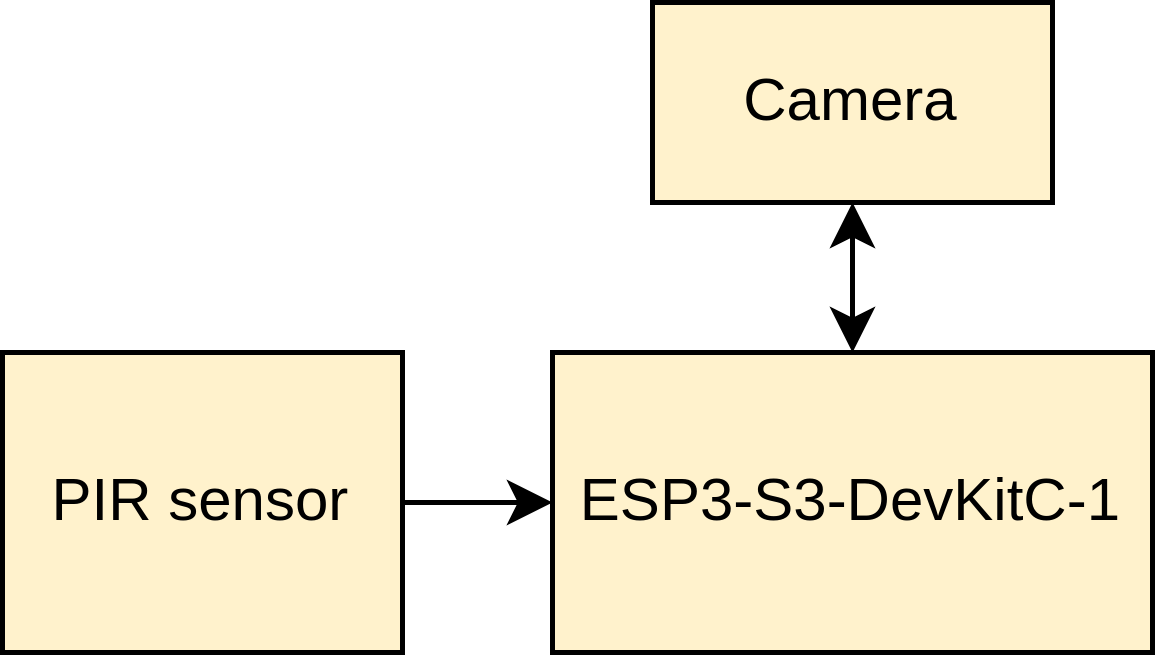
\includegraphics[width=0.5\textwidth]{./fig/blocks.png}
\caption{Diagrama en bloques del sistema}
\label{fig:blocks}
\end{figure}

\vspace{25px}

El sistema propuesto tiene como componente más importante una tarjeta de desarrollo ESP32-S3-DevKitC-1, cuyo elemento principal es un SoC (System on a Chip) ESP32-S3, que se encagará de ejecutar los modelos de DL, adquirir y procesar las imágenes obtenidas por la cámara, adquirir señales del sensor PIR (Passive InfraRed) y establecer comunicación con los servidores de AWS (Amazon Web Services) para enviar y recibir información. El sensor PIR ayuda a establer si cerca del sistema existe algún tipo de movimiento para ejecutar las tareas previstas con el menor uso de energía posible. La cámara tiene la función de obtener imágenes y digitalizarlas para ofrecerlas al SoC.

\section{2. Identificación y análisis de los interesados}
\label{sec:interesados}

\begin{table}[ht]
%\caption{Identificación de los interesados}
%\label{tab:interesados}
\begin{tabularx}{\linewidth}{@{}|l|X|X|l|@{}}
\hline
\rowcolor[HTML]{C0C0C0}
Rol           & Nombre y Apellido & Organización 			& Puesto 	\\ \hline
Responsable   & \authorname		& -        				& Alumno 	\\ \hline
Orientador    & \supname			& - 						& Director Trabajo final \\ \hline
Usuario final & -                 & -             			& -       	\\ \hline
\end{tabularx}
\end{table}

\begin{itemize}
	\item Orientador: Tiene la capacidad de ayudar al alumno a resolver los problemas técnicos y conceptuales que se presenten a lo largo del proyecto. Es exigente con los tiempos y la calidad del desarrollo del proyecto.
	\item Usuario final: No posee conocimientos sobre sistemas embebidos y las tecnologías utilizadas en el proyecto, y espera dispositivos de bajo costo económico.
\end{itemize}



\section{3. Propósito del proyecto}
\label{sec:proposito}

El propósito de este proyecto es diseñar e implementar un sistema embebido que mediante una cámara pueda detectar rostros humanos de las imágenes que obtiene con ayuda de uno o varios modelos de DL, para transmitir los resultados de sus predicciones a un servidor IoT.

Un propósito personal del autor es obtener conocimientos y experiencia sobre diseño e implementación de modelo de DL optmizados para sistemas embebidos.

\section{4. Alcance del proyecto}
\label{sec:alcance}

Este proyecto incluye:
\begin{itemize}
	\item Diseño e implementación del firmware del sistema embebido.
	\item Diseño e implementación de los modelos de DL para detección facial.
	\item Implementación del sistema embebido desarrollado dentro de una arquitectura IoT existente.
	\item Diseño e implementación de un dashboard para visualizar la información transmitida por el sistema embebido.
	\item Creación de documentación sobre datos técnicos y características del sistema embebido.
\end{itemize}

Este proyecto no incluye:
\begin{itemize}
	\item Desarrollo del PCB para el prototipo funcional del sistema embebido.
	\item Desarrollo de una aplicación para el usuario final.
\end{itemize}

\section{5. Supuestos del proyecto}
\label{sec:supuestos}

\begin{itemize}
	\item Se contará con el presupuesto necesario para obtener los componentes del proyecto.
	\item Se dedicarán al menos 2 horas diarias para la realización del proyecto.
	\item Se dispondrá de acesso a servicios en la nube para la realización de pruebas y puesta en marcha del proyecto.
\end{itemize}

\section{6. Requerimientos}
\label{sec:requerimientos}

El presente proyecto tiene dos tipos de requerimientos, funcionales y no funcionales. A continuación se citan los antes referidos.

\begin{enumerate}
	\item Requerimientos funcionales
		\begin{enumerate}
			\item El sistema debe conectarse a una red Wi-Fi existente a través de algún mecanismo de provisionamiento de credenciales de red.
			\item El sistema debe establecer comunicación con los servidores de AWS.
			\item El sistema debe ser alimentado mediante dos baterías AA de litio.
			\item El sistema debe poseer mecanismos de seguridad implementados tanto en hardware como en firmware para evitar su manipulación incorrecta.
			\item El sistema debe funcionar solamente si se detecta movimiento en el sector donde se encuentra instalada.
			\item El sistema debe, a través de uno o varios modelos de DL, detectar la cantidad de rostros humanos presentes en una fotografía obtenida por su cámara.
		\end{enumerate}
	\item Requerimientos no funcionales
		\begin{enumerate}
			\item El sistema debe tener un costo de desarrollo igual o menor a 200U\$S.
			\item El sistema debe tener documentación adecuada sobre su uso y desarrollo.
		\end{enumerate}
\end{enumerate}

\section{7. Historias de usuarios (\textit{Product backlog})}
\label{sec:backlog}

El criterio para determinar los \textit{storyboards} es el siguiente.

\begin{itemize}
	\item Complejidad
	\begin{itemize}
		\item Alto: 5
		\item Medio: 3
		\item Bajo: 1
	\end{itemize}
	\item Tiempo
	\begin{itemize}
		\item Alto: 5
		\item Medio: 3
		\item Bajo: 1
	\end{itemize}
	\item Recursos
	\begin{itemize}
		\item Alto: 5
		\item Medio: 3
		\item Bajo: 1
	\end{itemize}
\end{itemize}

\begin{enumerate}
	\item Como usuario quiero que la duración de las baterías sea al menos de 1 año para que no suponga un costo económico adicional muy alto en el futuro.
	\begin{itemize}
		\item Complejidad: 4
		\item Tiempo: 4
		\item Recursos: 4
	\end{itemize}
		\item Como usuario quiero poder visualizar la información que genera el sistema en un dashboard que pueda ser accedido mediante internet.
	\begin{itemize}
		\item Complejidad: 3
		\item Tiempo: 5
		\item Recursos: 2
	\end{itemize}
	\item Como usuario quiero que la configuración del sistema se realice en la menor cantidad posible de pasos para evitar complicaciones en su puesta en marcha.
	\begin{itemize}
		\item Complejidad: 2
		\item Tiempo: 3
		\item Recursos: 1
	\end{itemize}
	\item Como desarrollador del firmware quiero que el sistema esté basado en un RTOS (Real Time Operating System) para poder escalar la aplicación de manera más sencilla en el futuro.
	\begin{itemize}
		\item Complejidad: 3
		\item Tiempo: 2
		\item Recursos: 1
	\end{itemize}
	\item Como desarrollador del hardware quiero que el sistema se componga de la menor cantidad posible de componentes electrónicos para optmizar el proceso y tiempo de desarrollo.
	\begin{itemize}
		\item Complejidad: 4
		\item Tiempo: 5
		\item Recursos: 3
	\end{itemize}	
\end{enumerate}

\section{8. Entregables principales del proyecto}
\label{sec:entregables}

Los entregables del proyecto son:

\begin{itemize}
	\item Repositorio en Github con el código fuente.
	\item Prototipo de pruebas del sistema embebido.
	\item Informe final.
\end{itemize}

\section{9. Desglose del trabajo en tareas}
\label{sec:wbs}

\begin{enumerate}
\item Análisis y planificación preliminar (122 hs)
	\begin{enumerate}
		\item Planificar el proyecto. (38 hs)
		\item Investigar sobre sistemas similares. (24 hs)
		\item Recopilar y estudiar documentos de los componentes a utilizar. (30 hs)
		\item Planificar y diagramar la arquitectura a utilizar en el sistema (10 hs)
		\item Crear un repositorio en la nube para almacenar el código a desarrollar (2 hs)
	\end{enumerate}
	
\item Prototipo de pruebas (40 hs)
	\begin{enumerate}
		\item Importar los componentes del sistema. (12 hs)
		\item Probar la funcionalidad de todos los componentes del sistema individualmente. (26 hs)
		\item Construir el prototipo de pruebas y asegurar sus conexiones. (2 hs)
	\end{enumerate}
	
\item Firmware ( hs)
	\begin{enumerate}
		\item Elegir las herramientas para desarrollar el firmware. (hs)
		\item Instalar y configurar las herramientras para desarrollar el firmware. (hs)
		\item Desarrollar código para manejar la cámara del sistema. (hs)
		\item Desarrollar código para manejar la conectividad Wi-Fi del sistema. (hs)
		\item Desarrollar código para manejar el protocolo MQTT. (hs)
	\end{enumerate}
	
\item IoT (148 hs)
	\begin{enumerate}
		\item Estudiar e implementar los servicios de AWS necesarios para el sistema. (hs)
		\item Integrar los servicios de AWS implementados con el firmware desarrollado. (hs)
		\item Desarrollar código para integrar el modelo de ML en el sistema. (32 hs)
		\item Desarrollar una biblioteca de código para controlar la cámara del sistema. (24 hs)
		\item Desarrollar código para integrar la cámara del sistema con el modelo de ML. (12 hs)
		\item Probar el código desarrollado en el prototipo de pruebas. (10 hs)
	\end{enumerate}

\item DL (82 hs)
	\begin{enumerate}
		\item Realizar cursos sobre DL y visión artificial
. (hs)
		\item Investigar los modelos de DL aplicables al proyecto. (hs)
		\item Desarrollar los modelos de DL. (hs)
		\item Integrar los modelos de DL con el firmware desarrollado. (hs)
	\end{enumerate}

\item V\&V (48 hs)
	\begin{enumerate}
		\item Medir los parámetros eléctricos del sistema con instrumentación de laboratorio. (8 hs)
		\item Probar el sistema en un entorno de trabajo controlado. (36 hs)
		\item Analizar las experiencias de uso reportadas por los usuarios. (4 hs)
	\end{enumerate}
	
\item Cierre (106 hs)
	\begin{enumerate}
		\item Elaborar la memoria técnica del trabajo final. (80 hs)
		\item Elaborar la presentación del trabajo final. (26 hs)
	\end{enumerate}
\end{enumerate}

Cantidad total de horas: (612 hs)

\section{10. Diagrama de Activity On Node}
\label{sec:AoN}

El diagrama de actividades se puede observar en la figura \ref{fig:AoN}.

\begin{figure}[htpb]
\centering
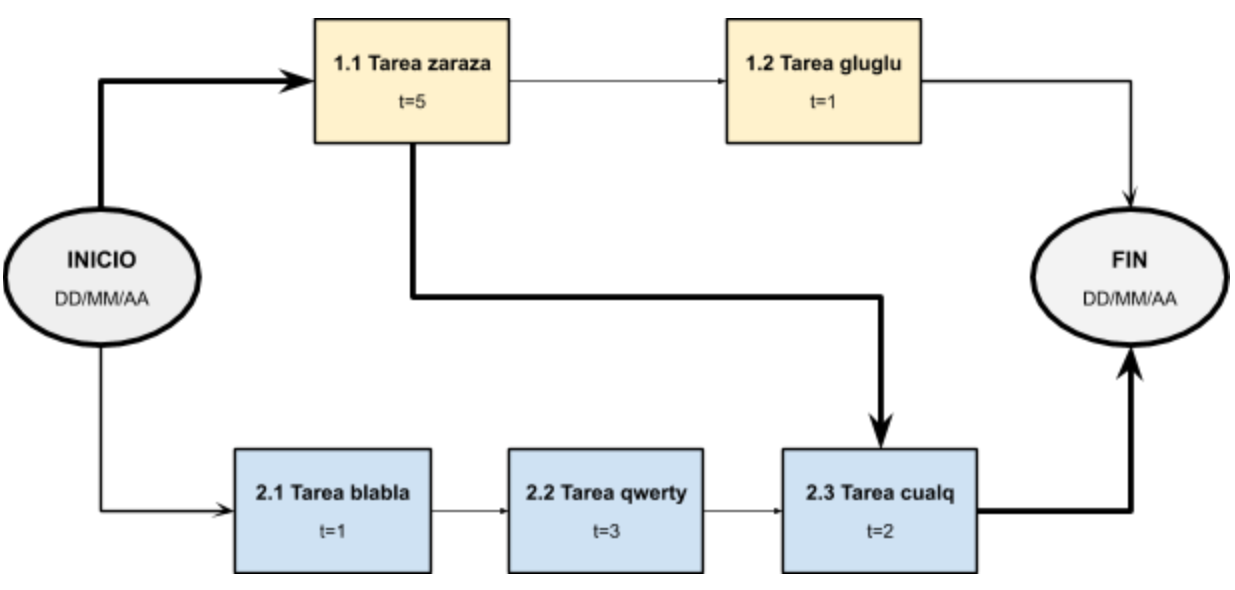
\includegraphics[width=.8\textwidth]{./fig/AoN.png}
\caption{Diagrama en \textit{Activity on Node}}
\label{fig:AoN}
\end{figure}

\section{11. Diagrama de Gantt}
\label{sec:gantt}

En la figura \ref{sec:gantt} se puede observar el diagrama de Gantt de este proyecto.

\begin{landscape}
\begin{figure}[htpb]
\centering
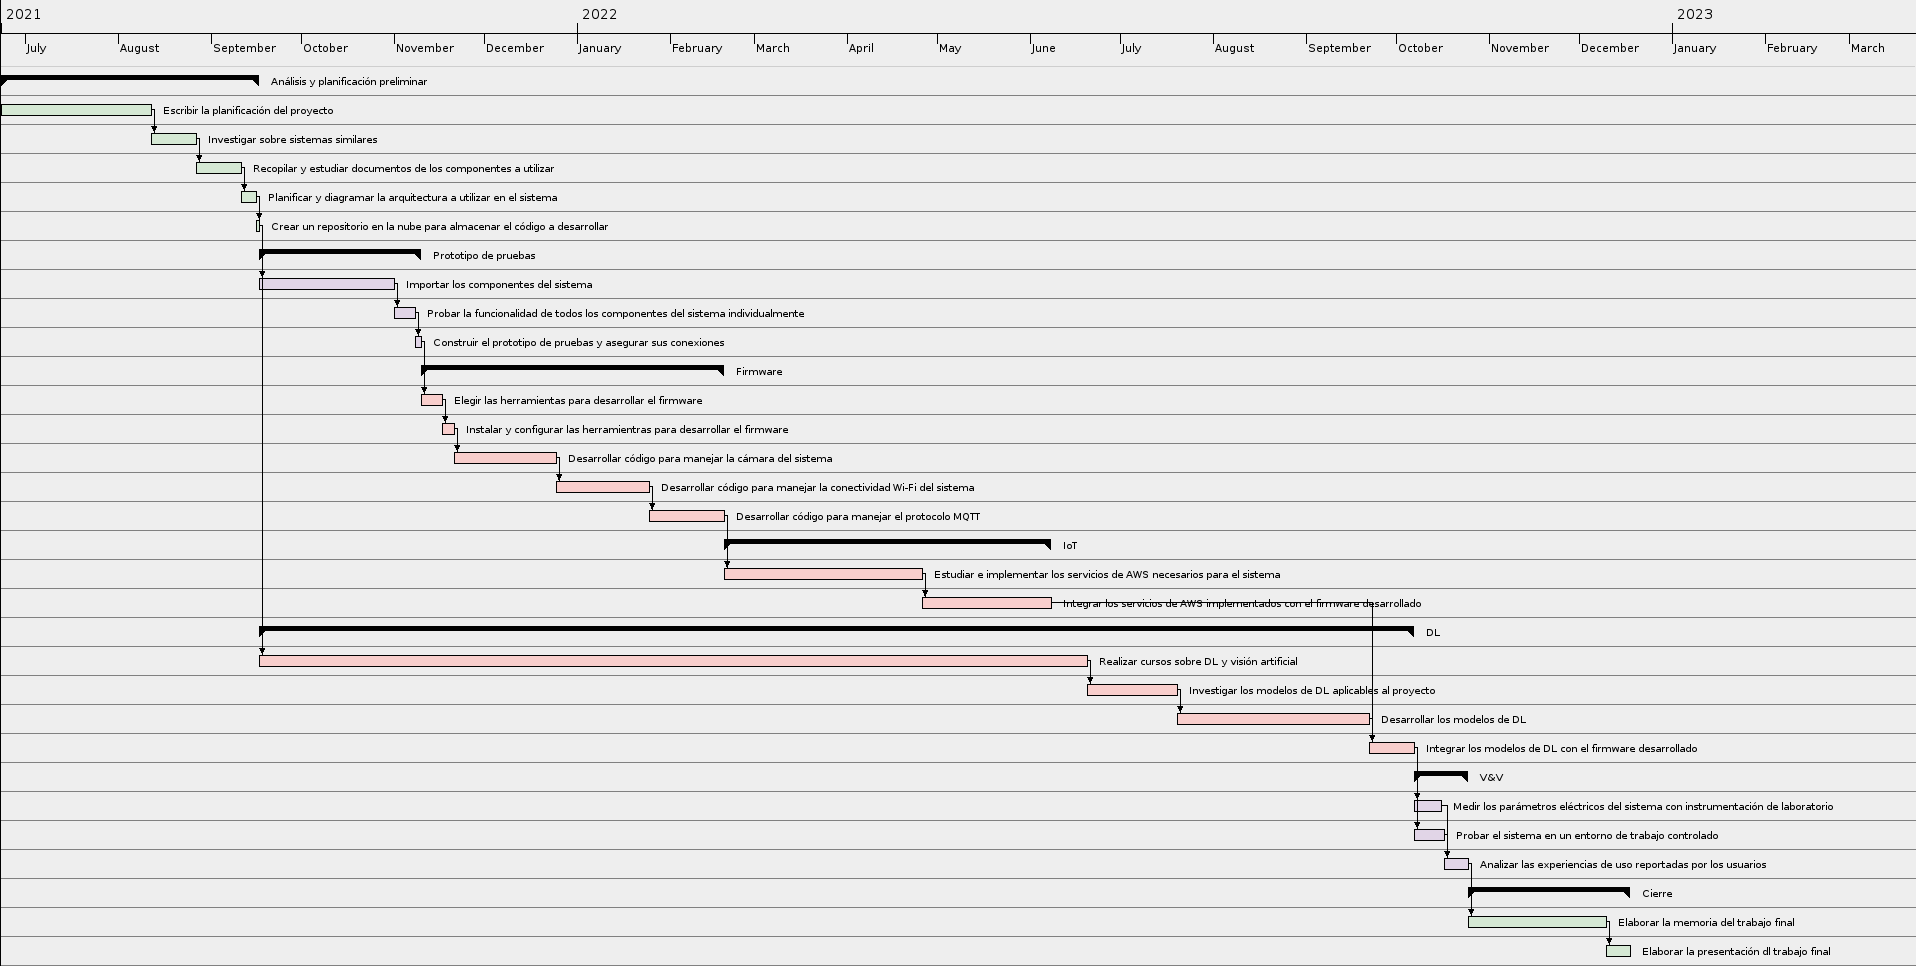
\includegraphics[height=.8\textheight]{./fig/gantt.png}
\caption{Diagrama de Gantt}
\label{fig:diagGantt}
\end{figure}

\end{landscape}



\section{12. Presupuesto detallado del proyecto}
\label{sec:presupuesto}

El presupuesto que se presenta en esta sección es un aproximado, ya que valores de los componentes que son parte del sistema embebido aún no fueron definidos. Por tanto, se consideran los costos más altos del mercado de componentes que cumplan las funciones requeridas. De esta manera se tiene un presupuesto suficiente para cumplir con el proyecto.

\begin{table}[htpb]
\centering
\begin{tabularx}{\linewidth}{@{}|X|c|r|r|@{}}
\hline
\rowcolor[HTML]{C0C0C0}
\multicolumn{4}{|c|}{\cellcolor[HTML]{C0C0C0}COSTOS DIRECTOS} \\ \hline
\rowcolor[HTML]{C0C0C0}
Descripción &
 \multicolumn{1}{c|}{\cellcolor[HTML]{C0C0C0}Cantidad} &
 \multicolumn{1}{c|}{\cellcolor[HTML]{C0C0C0}Valor unitario} &
 \multicolumn{1}{c|}{\cellcolor[HTML]{C0C0C0}Valor total} \\ \hline
\multicolumn{1}{|l|}{Placa de desarrollo ESP32-S3-DevKitC-1U-N8R8} &
\multicolumn{1}{|c|}{2} &
\multicolumn{1}{|c|}{15} &
\multicolumn{1}{|c|}{30}
  \\ \hline
\multicolumn{1}{|l|}{Módulo con cámara OV2640} &
\multicolumn{1}{|c|}{2} &
\multicolumn{1}{|c|}{11,99} &
\multicolumn{1}{|c|}{23,98}
  \\ \hline
\multicolumn{1}{|l|}{Sensor PIR IRA-S410ST01} &
\multicolumn{1}{|c|}{2} &
\multicolumn{1}{|c|}{3,49} &
\multicolumn{1}{|c|}{6,98}
  \\ \hline
\multicolumn{1}{|l|}{Amplificador operacional TLV8544} &
\multicolumn{1}{|c|}{2} &
\multicolumn{1}{|c|}{1,82} &
\multicolumn{1}{|c|}{3,64}
  \\ \hline
\multicolumn{1}{|l|}{Otros (cables, conectores, etc)} &
\multicolumn{1}{|c|}{2} &
\multicolumn{1}{|c|}{10} &
\multicolumn{1}{|c|}{20}
  \\ \hline
\multicolumn{3}{|c|}{SUBTOTAL} &
 \multicolumn{1}{c|}{84,6} \\ \hline
\rowcolor[HTML]{C0C0C0}
\multicolumn{4}{|c|}{\cellcolor[HTML]{C0C0C0}COSTOS INDIRECTOS} \\ \hline
\rowcolor[HTML]{C0C0C0}
Descripción &
 \multicolumn{1}{c|}{\cellcolor[HTML]{C0C0C0}Cantidad} &
 \multicolumn{1}{c|}{\cellcolor[HTML]{C0C0C0}Valor unitario} &
 \multicolumn{1}{c|}{\cellcolor[HTML]{C0C0C0}Valor total} \\ \hline
\multicolumn{1}{|l|}{50\% del costo directo} &
\multicolumn{1}{|c|}{1} &
\multicolumn{1}{|c|}{42,3} &
\multicolumn{1}{|c|}{42,3}
  \\ \hline
\multicolumn{3}{|c|}{SUBTOTAL} &
 \multicolumn{1}{c|}{42,3} \\ \hline
\rowcolor[HTML]{C0C0C0}
\multicolumn{3}{|c|}{TOTAL} &
\multicolumn{1}{|c|}{126,9}
  \\ \hline
\end{tabularx}%
\end{table}

Los valores expuestos en la tabla anterior están expresados en dólares americanos (U\$S). Esto es por que todos los componentes serán adquiridos de el distribuidor Mouser, ubicado en Estados Unidos.

\section{13. Gestión de riesgos}
\label{sec:riesgos}

a) Identificación de los riesgos y estimación de sus consecuencias:

Riesgo 1: Imposibilidad de obtener los componentes necesarios.
\begin{itemize}
	\item Severidad (S): 7. El sistema podría no funcionar de acuerdo a lo planificado.
	\item Probabilidad de ocurrencia (O): 3. Si no se encuentran los componentes en el mercado local, estos pueden ser importados
\end{itemize}  

Riesgo 2: El tamaño de los modelos de DL desarrollados puede sobrepasar la cantidad de memoria disponible.
\begin{itemize}
	\item Severidad (S): 9. Si lso modelos de DL no pueden ser almacenados en la memoria disponible, el sistema no podría realizar las funciones para las que fue planificado.
	\item Ocurrencia (O): 7. El tamaño de los modelos de DL alcanzarán un tamaño no adecuado en función de su complejidad y su optimización.
\end{itemize}

Riesgo 3: Imposibilidad de contar con instrumentación de laboratorio.
\begin{itemize}
	\item Severidad (S): 3. Las mediciones de alta precisión son para contar con datos técnicos exactos, que ayudarán a desarrollar una versión comercial del sistema posteriormente.
	\item Ocurrencia (O): 2. En el lugar de residencia del autor se cuenta con un laboratorio de electrónica que funciona regularmente y está abierto al público previa aceptación de los encargados.
\end{itemize}

Riesgo 4: Imposibilidad de contar con los recursos económicos necesarios.
\begin{itemize}
	\item Severidad (S): 10. No contar con el dinero necesario para comprar los componentes del sistema impediría la realización del proyecto.
	\item Ocurrencia (O): 2. El presupuesto requerido para el proyecto es relativamente bajo y son recursos que ya se tienen reservados.
\end{itemize}

Riesgo 5: Falta de tiempo para concluir el proyecto.
\begin{itemize}
	\item Severidad (S): 5. Si el proyecto no se concluye en las fechas planificadas, existe la posibilidad de que se retrase indefinidamente si se presentan otros proyectos más de mayor prioridad.
	\item Ocurrencia (O): 6. Por cuestiones tanto laborales como familiares el proyecto podría retrasarse de manera imprevista.
\end{itemize}

b) Tabla de gestión de riesgos:      (El RPN se calcula como RPN=SxO)

\begin{table}[htpb]
\centering
\begin{tabularx}{\linewidth}{@{}|X|c|c|c|c|c|c|@{}}
\hline
\rowcolor[HTML]{C0C0C0}
Riesgo & S & O & RPN & S* & O* & RPN* \\ \hline
Imposibilidad de obtener los componentes necesarios & 7 & 3 & 21 & - & - & -\\ \hline
El tamaño de los modelos de DL desarrollados puede sobrepasar la cantidad de memoria disponible & 9 & 7 & 63 & 9 & 2 & 18\\ \hline
Imposibilidad de contar con instrumentación de laboratorio & 3 & 2 & 6 & - & - & -\\ \hline
Imposibilidad de contar con los recursos económicos necesarios & 10 & 2 & 20 & - & - & -\\ \hline
Falta de tiempo para concluir el proyecto & 5 & 6 & 30 & 5 & 4 & 20\\ \hline
\end{tabularx}%
\end{table}

Criterio adoptado:
Se tomarán medidas de mitigación en los riesgos cuyos números de RPN sean mayores a 25.

c) Plan de mitigación de los riesgos que originalmente excedían el RPN máximo establecido:
Riesgo 2: Se realizará un curso de ML en microcontroladores durante el periodo de vacaciones.
\begin{itemize}
	\item Severidad (S): 9. Este riesgo sigue siendo muy severo por más conocimientos de ML que se posean.
	\item Ocurrencia (O): 2. Con los conocimientos adecuados sobre ML en microcontroladores se pueden optimizar estos algoritmos, de tal forma que pueden adaptarse a la cantidad de memoria del microcontrolador a utilizar. \\ \\
\end{itemize}
Riesgo 5: Durante el tiempo planificado del proyecto se trabajarán los fines de semana y feriados 4 horas diarias.
\begin{itemize}
	\item Severidad (S): 5. La severidad no se ve afectada por la medida de mitigación.
	\item Ocurrencia (O): 4. Las horas extras que se destinarán al proyecto podrían asegurar su conclusión en el tiempo planificado. Su ocurrencia baja muy poco porque no se descarta la posibilidad de que surjan imprevistos que retrasen el proyecto.
\end{itemize}

\section{14. Gestión de la calidad}
\label{sec:calidad}



\begin{enumerate}
	\item Requerimientos funcionales
		\begin{itemize}
			\item Req \#1.1: el sistema debe conectarse a una red Wi-Fi existente a través de algún mecanismo de aprovisionamiento de credenciales de red.

			\begin{itemize}
				\item Verificación: conectar el sistema a una red Wi-Fi existente a través de el mecanismo de aprovisionamiento de credenciales de red y comprobar a través de la salida de monitor del sistema.
				\item Validación: conectar el sistema a una red Wi-Fi existente mediante una aplicación destinada para esto y comprobar su conexión a internet en la plataforma de AWS.
			\end{itemize}

		\end{itemize}
		
		\begin{itemize}
			\item Req \#1.2: El sistema debe establecer comunicación con los servidores de AWS.

			\begin{itemize}
				\item Verificación: mediante las herramientas de AWS para probar el protocolo MQTT, comprobar que los mensajes enviados desde el sistema son recepcionados correctamente.
				\item Validación: con ayuda de un dashboard visualizar la información del sistema.
			\end{itemize}
		\end{itemize}
		
		\begin{itemize}
			\item Req \#1.3: el sistema debe ser alimentado mediante dos baterías AA de litio.

			\begin{itemize}
				\item Verificación: con ayuda de un multímetro de precisión medir que los parámetros eléctricos requeridos por los componentes del sistema sean los requeridos por sus datasheets.
				\item Validación: visualizar el buen funcionamiento del sistema a través del LED RGB del sistema.
			\end{itemize}

		\end{itemize}
		
		\begin{itemize}
			\item Req \#1.4: el sistema debe poseer mecanismos de seguridad implementados tanto en hardware como en software para evitar su manipulación incorrecta.

			\begin{itemize}
				\item Verificación: mediante herramientas proporcionadas por el fabricante de la tarjeta de desarrollo, comprobar que los sectores de memoria dedicados a la seguridad funcionen correctamente.
				\item Validación: intentar leer la memoria de programa del sistema y comprobar que no es posible.
			\end{itemize}

		\end{itemize}
		
		\begin{itemize}
			\item Req \#1.5: el sistema debe funcionar solamente si se detecta movimiento en el sector donde se encuentra instalada.

			\begin{itemize}
				\item Verificación: con ayuda de la salida de monitor del sistema comprobar el estado del sistema y la detección de movimiento a través del sensor PIR.
				\item Validación: comprobar que el LED RGB del sistema se active por el movimiento de algún cuerpo que se encuentre en el área de detección del sistema.
			\end{itemize}

		\end{itemize}
				
		\begin{itemize}
			\item Req \#1.6: el sistema debe, a través de uno o varios modelos de DL, detectar la cantidad de rostros humanos presentes en una fotografía obtenida por su cámara.

			\begin{itemize}
				\item Verificación: probar los algoritmos de DL con un banco de pruebas compuesto por imágenes similares a las que serán adquiridas en un entorno real de trabajo, y comprobar su precisión con herramientas para la medición de métricas.
				\item Validación: probar el sistema en un entorno real de trabajo y monitorear los datos en los servidores de AWS.
			\end{itemize}

		\end{itemize}
		
	\item Requisitos no funcionales
	
		\begin{itemize}
			\item Req \#2.1: el sistema deberá tener un costo de desarrollo igual o menor a 200U\$S.

			\begin{itemize}
				\item Verificación: realizar la suma de los costos de cada componente para determinar que no se superó el presupuesto previamente propuesto.
				\item Validación: realizar un detalle de los costos del sistema.
			\end{itemize}

		\end{itemize}
		
		\begin{itemize}
			\item Req \#2.2: el sistema deberá tener documentación adecuada sobre su uso y desarrollo.

			\begin{itemize}
				\item Verificación: comprobar que los datos técnicos de los documentos sean consistentes con los datasheets y application notes de los componentes utilizados.
				\item Validación: presentar los documentos del proyecto a los directos interesados (director del trabajo, docentes y jurados).
			\end{itemize}

		\end{itemize}

\end{enumerate}

\section{15. Procesos de cierre}   
\label{sec:cierre}

Establecer las pautas de trabajo para realizar una reunión final de evaluación del proyecto, tal que contemple las siguientes actividades:

\begin{itemize}
	\item Pautas de trabajo que se seguirán para analizar si se respetó el Plan de Proyecto original:
		\begin{itemize}
			\item Responsable: Mauricio Barroso Benavides.
			\item Actividad: evaluar si se cumplieron los requerimientos del proyecto y las fechas planificadas.
		\end{itemize}
	\item Identificación de las técnicas y procedimientos útiles e inútiles que se emplearon, y los problemas que surgieron y cómo se solucionaron:
		\begin{itemize}
			\item Responsable: Mauricio Barroso Benavides.
			\item Actividad: evaluar las herramientas y metodologías para el desarollo de software y hardware del proyecto, para establecer las técnicas y procedimientos que se seguirán en proyectos futuros.
		\end{itemize}
	\item Indicar quién organizará el acto de agradecimiento a todos los interesados, y en especial al equipo de trabajo y colaboradores:
		\begin{itemize}
			\item Responsable: Mauricio Barroso Benavides.
			\item Actividad: agradecer públicamente a los profesores y responsables de la maestría, y a todos los involucrados en la realización del proyecto durante la defensa formal del mismo.
		\end{itemize}
\end{itemize}

\end{document}


